% System Design Project (SDP)
% Albert-Ludwigs-Universitaet Freiburg
% WS 2021 / 2022
% Project Report
\documentclass[12pt]{article}
\usepackage[utf8]{inputenc}
%\usepackage{ngerman}
\usepackage[ngerman]{babel}

\usepackage{geometry}
\geometry{a4paper, top=3cm, bottom=3cm}

\usepackage{xcolor}
\usepackage{graphicx}

\usepackage{hyperref}
\hypersetup{hidelinks}

\usepackage{float}
\usepackage{subfigure}

\usepackage{csquotes}

%%%%%%%%%%%%%%%%%%%%%%%%%%%%%%%%%%%%%%%%%%%%%%
%        Document settings and title         %
%%%%%%%%%%%%%%%%%%%%%%%%%%%%%%%%%%%%%%%%%%%%%%
% In German, new paragraphs are not indented
\setlength{\parindent}{0cm}

% Define new command for red color emphasis
\newcommand{\red}[1]{\textcolor{red}{#1}}

% Title section
\title{
  \vspace{2cm}
  \Huge System Design Projekt \\[0.2cm]
  \LARGE Abschlussbericht WS 2021/2022
}
\author{\Large VORNAME NACHNAME}
\date{ \today }

%%%%%%%%%%%%%%%%%%%%%%%%%%%%%%%%%%%%%%%%%%%%%%
%            Document starts here            %
%%%%%%%%%%%%%%%%%%%%%%%%%%%%%%%%%%%%%%%%%%%%%%
\begin{document}
\maketitle  % Inserts the title into document
\vspace{0.25cm}

% ============================================
% CONCEPT OF THE ROBOT
\section{Roboterkonzept}
% Beschreiben Sie einleitend das Grundkonzept Ihres Roboters und wie Sie vorhaben, die jeweiligen Teilaufgaben zu lösen. Dies muss, wenn es auf die Bauweise ankommt, mit jeweils mindestens einem Foto, wie in Abbildung~\ref{Figure:Front} und~\ref{Figure:Side} bzw. in Abbildung~\ref{Figure:Sensors} gezeigt, illustriert werden.
% Tipp: Mit geschützten Leerzeichen ($\sim$) können Zeilenumbrüche verhindert werden!

Der Roboter verfügt über zwei direkt gegenüberliegende, unabhängig von einander angetriebene Achsen mit größeren Rädern. Diese werden durch eine zusätzliche Achse mit einem kleinen Rad am hinteren Ende des Fahrzeugs unterstützt. Beide sind in Abbildung~\ref{Figure:Side} deutlich zu erkennen. Auf einem Grundgerüst liegt der NXT-Mikrocontroller orthogonal zur Fahrtrichtung auf. An ihm, sowie an weiteren Streben ist die Sensorkonstruktion (Abbildungen~\ref{Figure:Front}~und~\ref{Figure:Sensors}) befestigt.

\subsection{Linienverfolgung}

Zur Linienverfolgung besitzt der Roboter an seiner Front \textit{drei Lichtsensoren} (siehe Abbildung~\ref{Figure:Front}), davon einen in der Mitte, der die Leitlinie entlang der Strecke verfolgt. Ein linker und ein rechter Sensor haben je einen Abstand von ca $5~cm$ zum mittleren Sensor, sie verfolgen die Umgebung neben der Fahrlinie und dienen der Erkennung von Kurven. Die Linien werden erkannt indem der Sensorwert gegen einen festgelegten Grenzwert verglichen wird.

\subsection{Schranke}

Zur Erkennung der Schranke sieht das Roboterkonzept eine universelle \textit{Erkennung von Objekten auf der Strecke} mittels des frontal angebrachten \textit{Ultraschallsensors}, wie in Abbildung~\ref{Figure:Front} zu sehen vor. Mit ihm ermittelt das Gerät den Abstand zu Objekten vor ihm. Wenn dieser Wert einen Grenzwert unterschreitet, wird abgewartet solange bis die Strecke wieder frei ist. Dann setzt der Roboter seine Fahrt fort.

\subsection{Entscheidung}

Die Entscheidung bei Weggabelungen fällt der Roboter nicht durch ein dezidiertes Verfahren sondern lediglich dadurch, dass zuerst geprüft wird, ob eine Linkskurve anhand der Sensorwerte möglich ist bevor dasselbe für eine Rechtskurve geschieht. Somit wählt der Roboter \textit{bevorzugt den linken Weg}.

\subsection{Lücken}

Wenn der Roboter anhand der Werte der Lichtsensoren keine Fahrlinie mehr ermitteln kann, fährt er \textit{geradeaus weiter} und beginnt eine \textit{Zeitzählung}. Überschreitet die Zeit, die ohne Fahrlinie gefahren wird einen festgelegten Grenzwert bricht der Roboter die Fahrt ab und kehrt rückwärts zur Fahrlinie zurück. Dieses Verfahren kommt auch beim Linienende zum Einsatz.

\subsection{Enge Kurven}

Der \textit{mittlere Lichtsensor} dient im Falle einer Kurve zur \textit{Abschätzung des Kurvenradius}. Wenn einer der äußeren Sensoren anschlägt und das Gerät folglich um eine Kurve fährt, so wird auch der mittlere Sensor berücksichtigt. Wenn er ebenfalls anschlägt wird weniger scharf um die Kurve gefahren. Dies realisiert sich über die Zugkraft des Motors im Kurveninneren. Er wird bei einer weiten Kurve nur gedrosselt, bei einer scharfen Kurve ganz abgeschaltet.

% ============================================
% IMAGES OF THE ROBOT'S CONSTRUCTION
% \clearpage
\quad % Separate images and subsections
\vspace{2cm}

% Subfigure with two images
\begin{figure}[H]
  \centering
  \subfigure[Frontansicht]{
    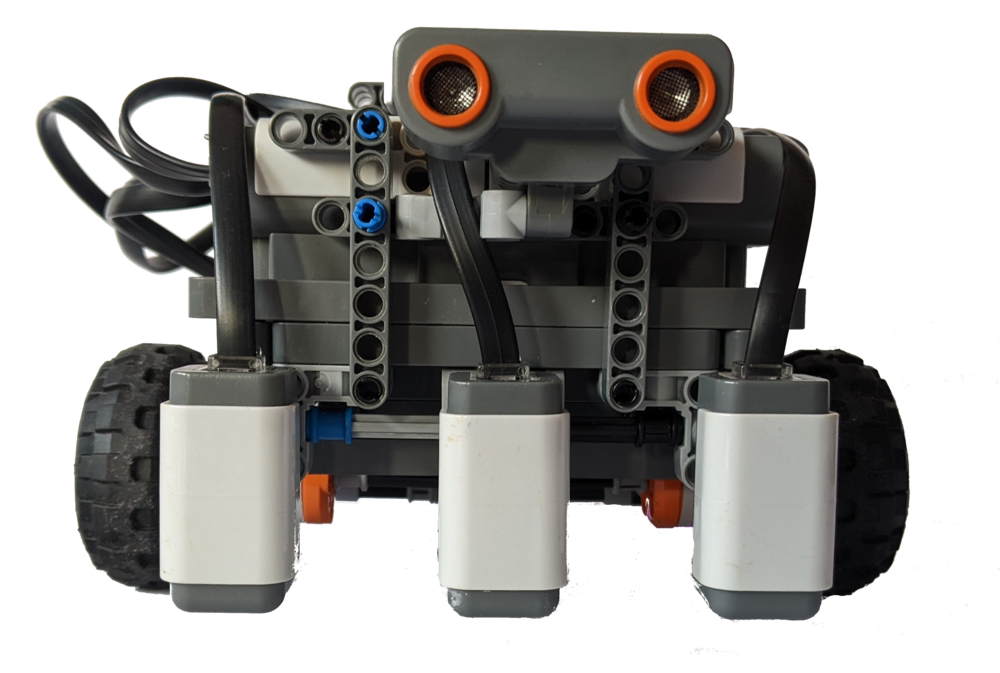
\includegraphics[width=0.47\textwidth]{Front.png}
    \label{Figure:Front}
  }
  \subfigure[Seitenansicht]{
    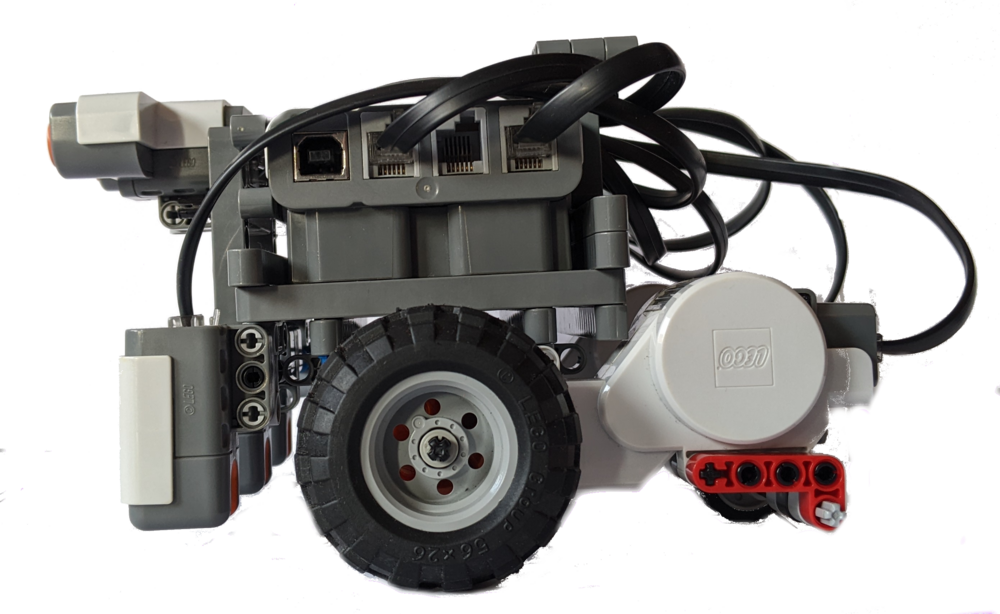
\includegraphics[width=0.47\textwidth]{Side.png}
    \label{Figure:Side}
  }
  \caption{Bilder der Front- und Seitenansicht des NXT Roboters.}
  \label{Figure:RobotPics}  % Labels are used for referencing with \ref{}
\end{figure}

% Single centered image
\begin{figure}[H]
  \centering
  % Image with 70% of document width.
  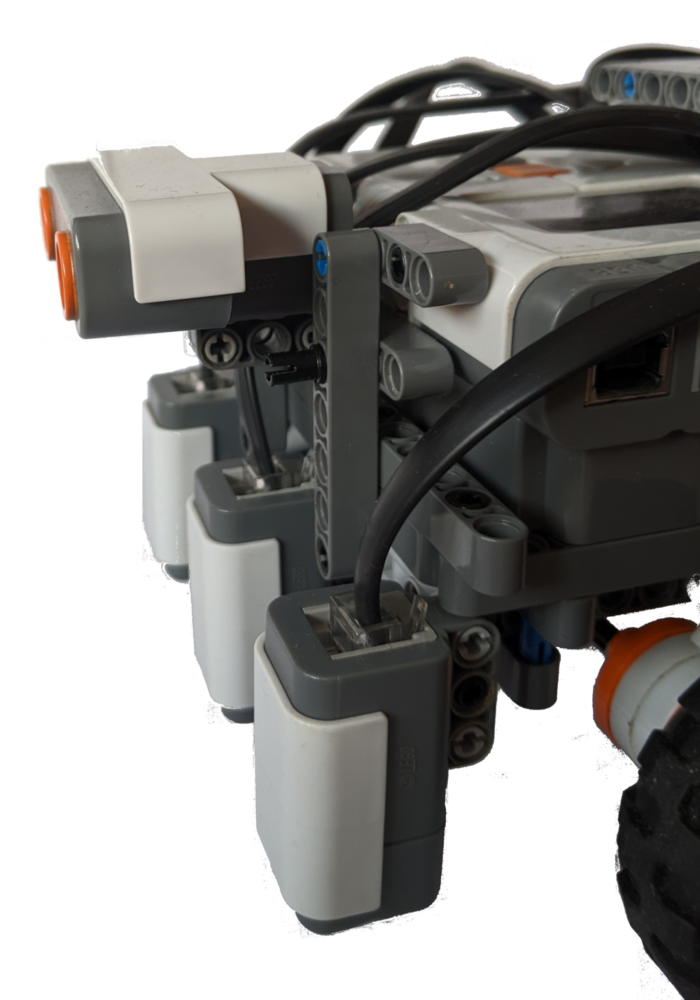
\includegraphics[width=0.47\textwidth]{Sensors.png}
  \caption{Seitenansicht der Sensor-Vorrichtung.}
  \label{Figure:Sensors}
\end{figure}

\quad
%\clearpage

% ============================================
% ROBOT SOFTWARE
\section{Softwarekonzept}
% Beschreiben Sie hier, wie Sie die Programmierung des Roboters umgesetzt haben und erklären Sie im Detail z.B. die State Machine und den PID-Regler.

Das Softwarekonzept des Roboters zeichnet sich durch eine klare Trennung verschiedener Abläufe aus, deren Sequenz in \texttt{task main()} definiert ist. Nach Initialisierung besteht das Programm aus den Grundoperationen \texttt{readSensors()} zum Auslesen, Interpretieren und Speichern der Sensorwerte, \texttt{show()} zur Ausgabe des Zustands und der Sensorwerte auf dem Display und \textit{Engine Control}, Funktionen zur Steuerung der Motoren. Diese Operationen laufen im \textit{\enquote{Course correction loop}} zusammen, einer Endlosschleife die den aktuellen Stand des Roboters mit \texttt{readSensors()} (und dem Zähler \texttt{cyclesNoLine}) ermittelt und mit den Funktionen des \textit{Engine Control} daraus Konsequenzen für die Fahrt des Robotes ableitet, die das Gerät dann für einen \textit{\enquote{Zyklus}} (\texttt{TTL}) beibehält. Wird das Ende der Strecke erkannt, bricht die Schleife ab und das Programm endet.

% ============================================
% PROJECT ISSUES
\section{Fehleranalyse}
% Beschreiben Sie die Herausforderungen, die Ihnen bei der Entwicklung begegnet sind. Welche Probleme hatten Sie bisher beim Bau der Hardware und bei der Bewältigung der einzelnen Aufgaben? Zu welchen Lösungen sind Sie gekommen?

Ein großes Problem stellten die geringe Menge an LEGO-Bauteilen insbes. Verbindungspins und viele defekte Bauteile im Kasten dar. Die Windowssoftware \textit{Bricx-CC} konnte mithilfe einer Virtuellen Maschine und Bus-Passthrough des Bluetooth-Controllers auch unter Linux ohne große Anstrengungen angewendet werden. Beim Bau und bei der Programmierung ergaben sich keine größeren Probleme.

\end{document}
